\section{Exkurs}
\begin{frame}[fragile]
	\frametitle{Exkurs}
\huge Exkurs
\end{frame}

\begin{frame}
\frametitle{Vagrant}
	\begin{block}{Vagrant}
		Erlaubt einfache und reproduzierbare Erstellung von Entwicklungsumgebungen.
    Provisionierung auf Basis von Virtual Box, VMWare, AWS ... Nutzung von Tools
    wie Chef, Puppet, Shell-Skripte
	\end{block}
\end{frame}

\begin{frame}
\frametitle{Docker}
	\begin{block}{Docker}
		Docker ist eine Plattform zur Virtualisierung in Containern.
	\end{block}
  \bigskip
  \begin{itemize}
    \item Container sind Software auf Filesystem
    \item Nutzen Kernel des Hosts
    \item Sind Prozesse auf Host
  \end{itemize}
\end{frame}

\subsection{Continous Integration / Delivery mit Docker}

\begin{frame}
\frametitle{Continous Integration / Delivery mit Docker}
  \huge Continous Integration / Delivery mit Docker
\end{frame}

\begin{frame}
\frametitle{Setup}
  \center
  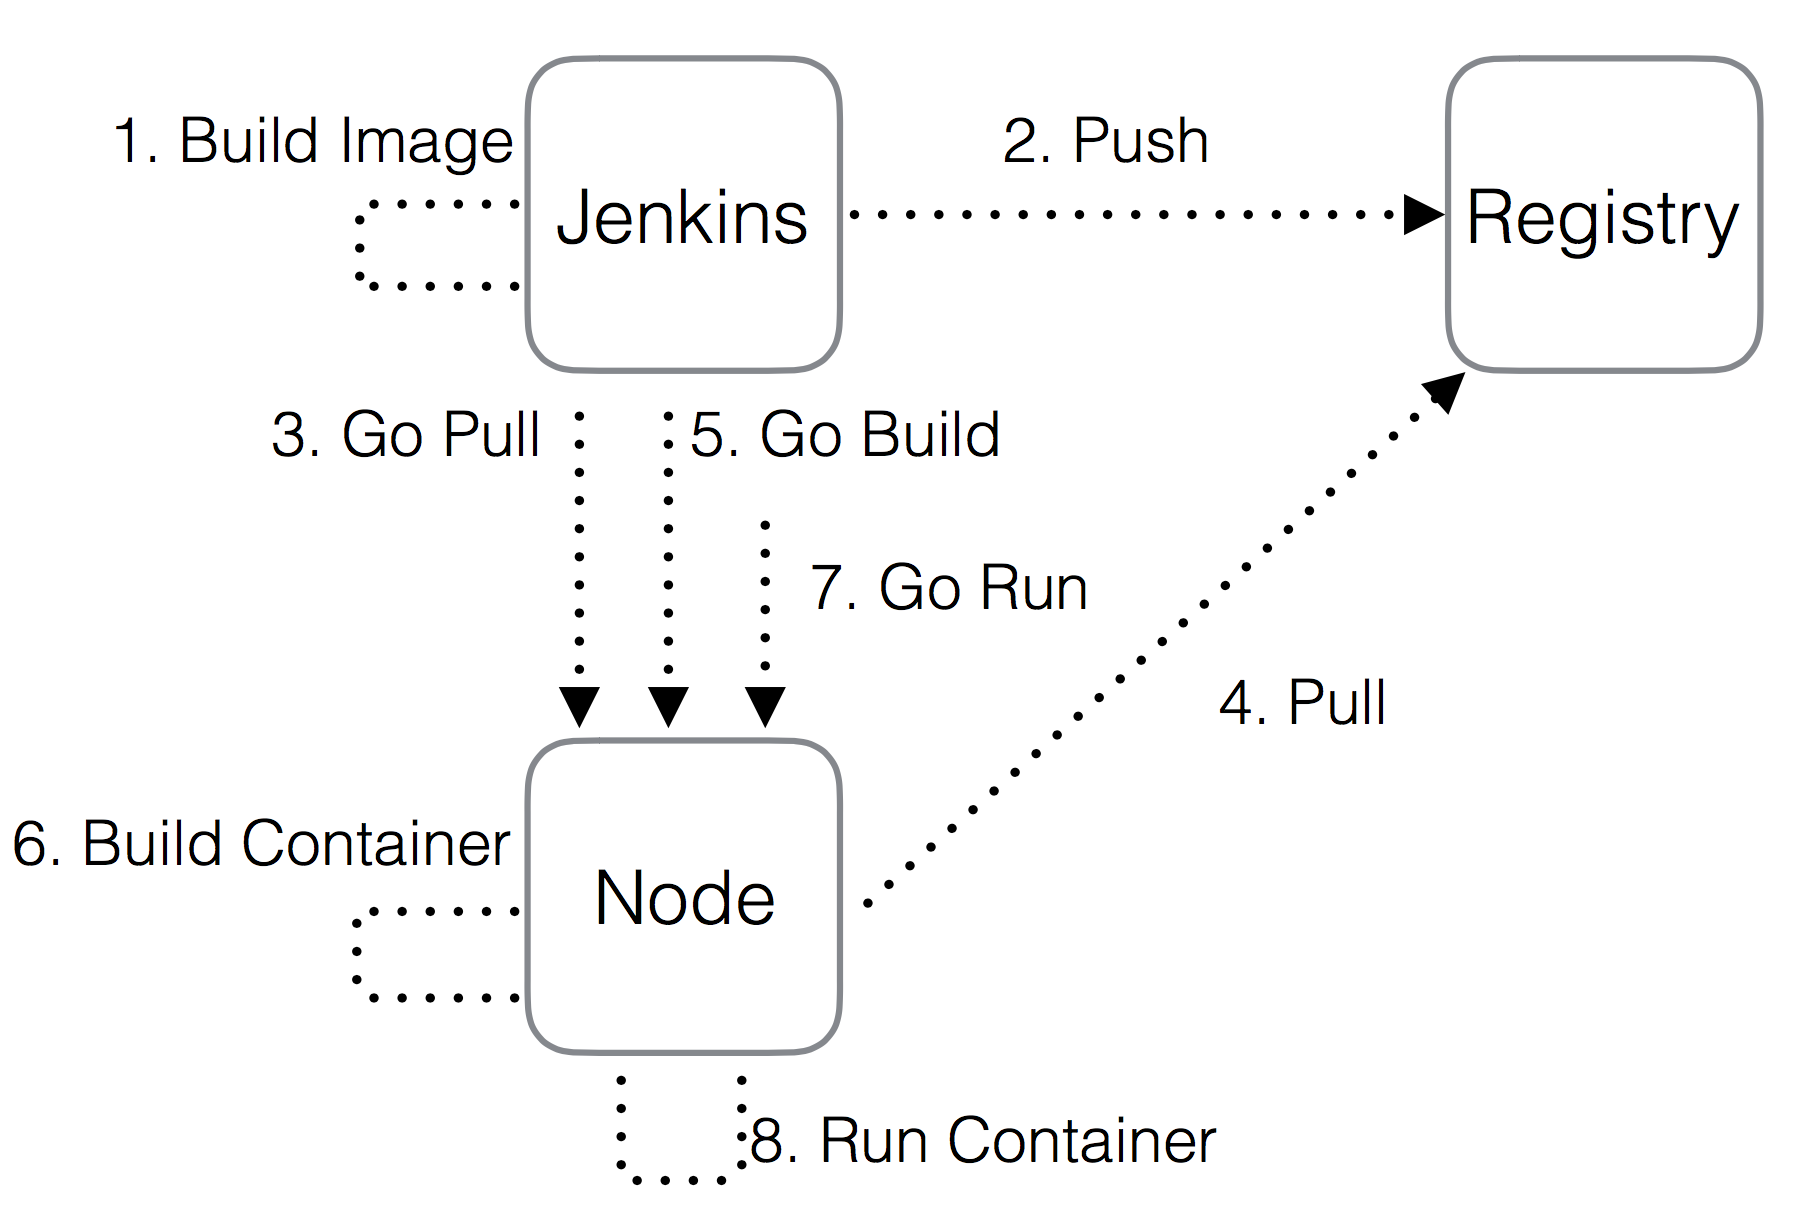
\includegraphics[width=1\textwidth,
  keepaspectratio=true]{bilder/ci_cd_process.png}
\end{frame}

\subsection{Data Science mit Apache Spark und Jupyter}

\begin{frame}
\frametitle{Data Science mit Apache Spark und Jupyter}
  \huge Data Science mit Apache Spark und Jupyter
\end{frame}

\begin{frame}
\frametitle{Setup}
  \center
  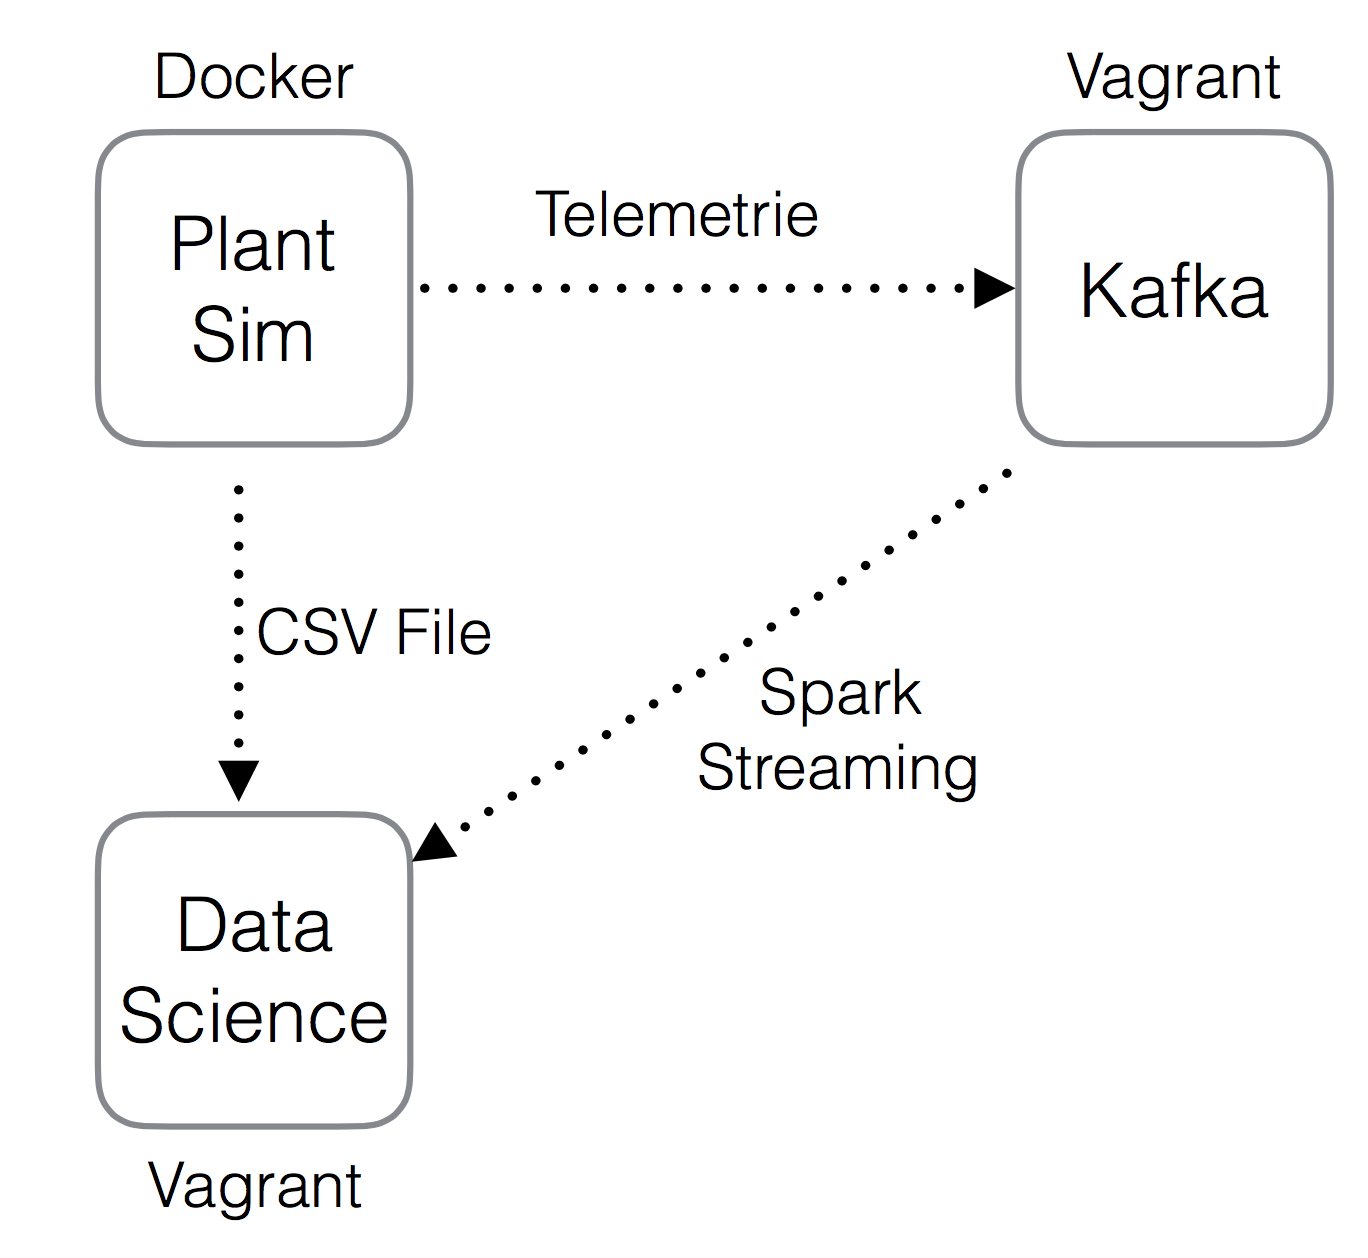
\includegraphics[width=0.9\textwidth,
  keepaspectratio=true]{bilder/data_science_blank.png}
\end{frame}

\begin{frame}
\frametitle{Setup}
  \center
  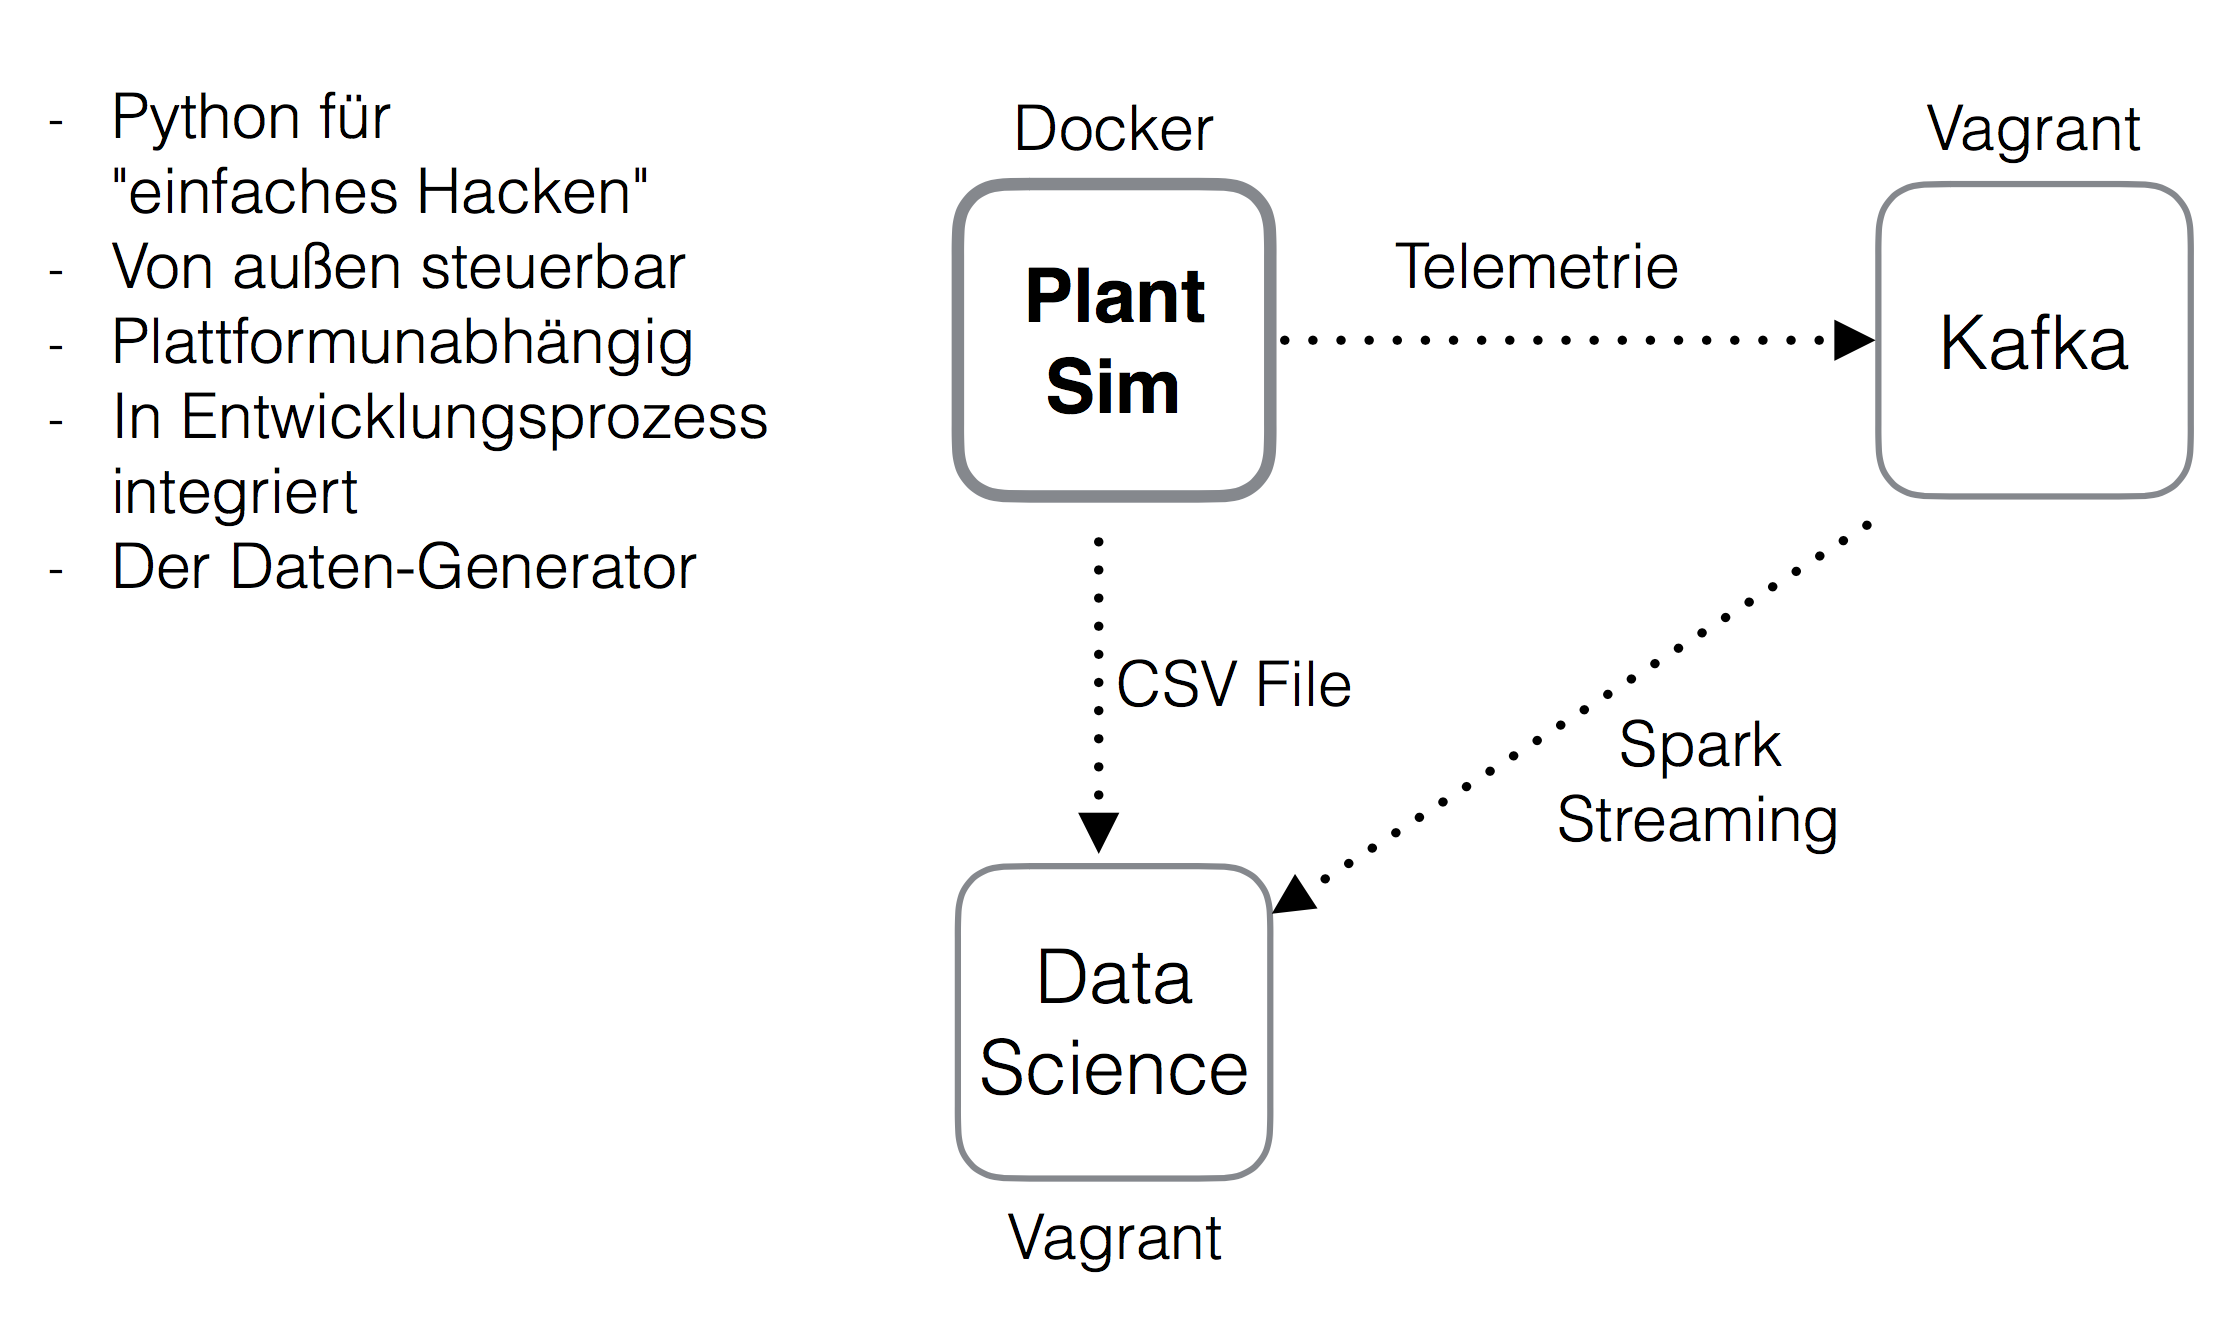
\includegraphics[width=1\textwidth,
  keepaspectratio=true]{bilder/data_science_sim.png}
\end{frame}

\begin{frame}
\frametitle{Setup}
  \center
  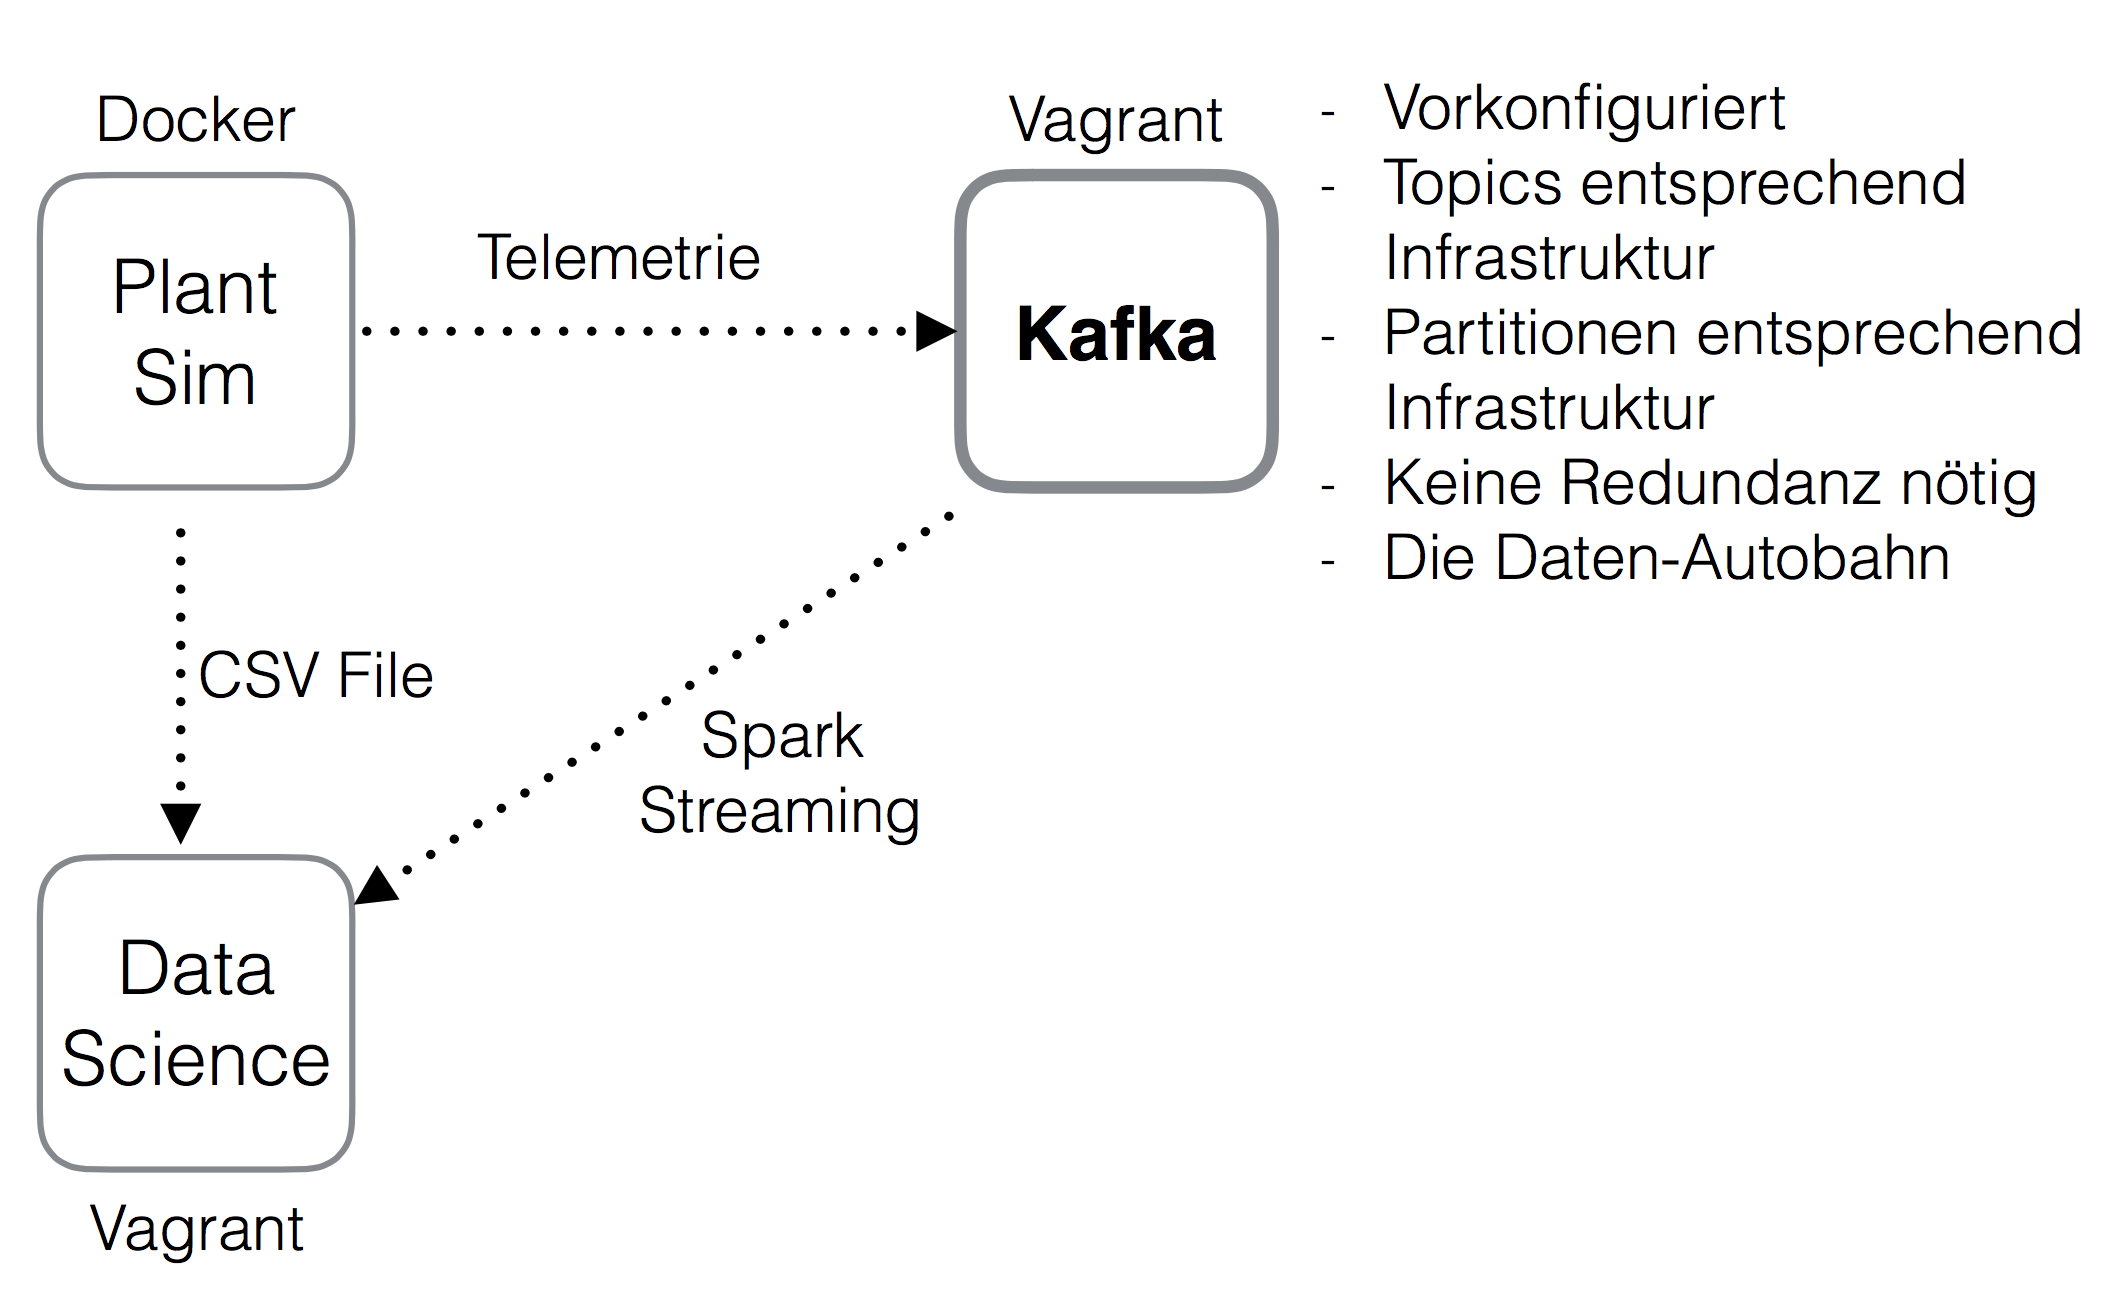
\includegraphics[width=1\textwidth,
  keepaspectratio=true]{bilder/data_science_kafka.png}
\end{frame}

\begin{frame}
\frametitle{Setup}
  \center
  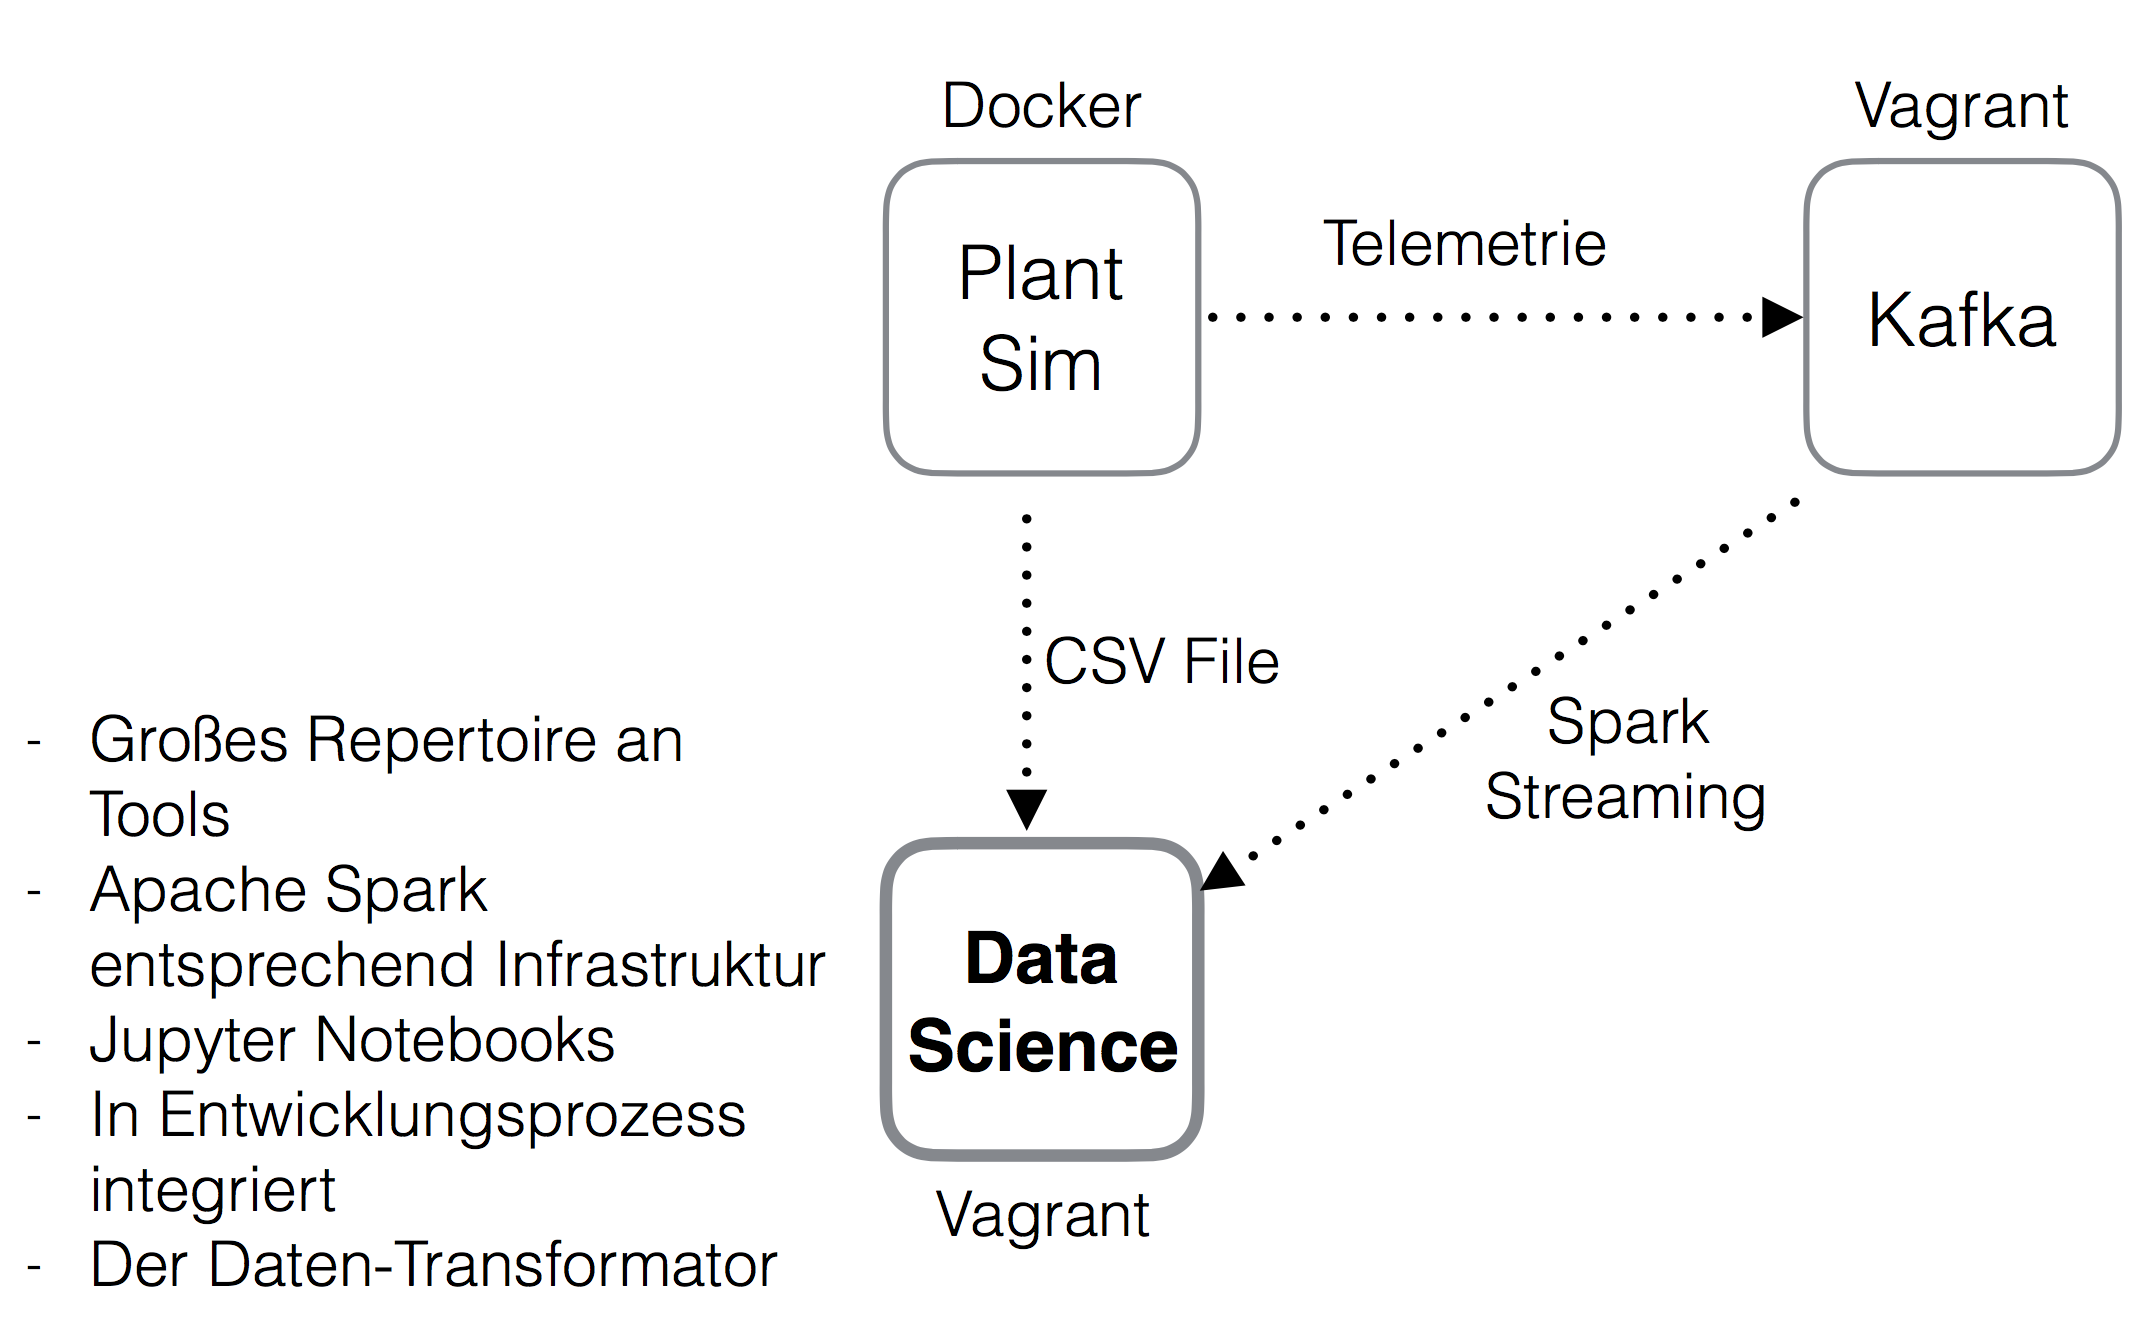
\includegraphics[width=1\textwidth,
  keepaspectratio=true]{bilder/data_science_spark.png}
\end{frame}

\begin{frame}
\frametitle{Setup}
  \center
  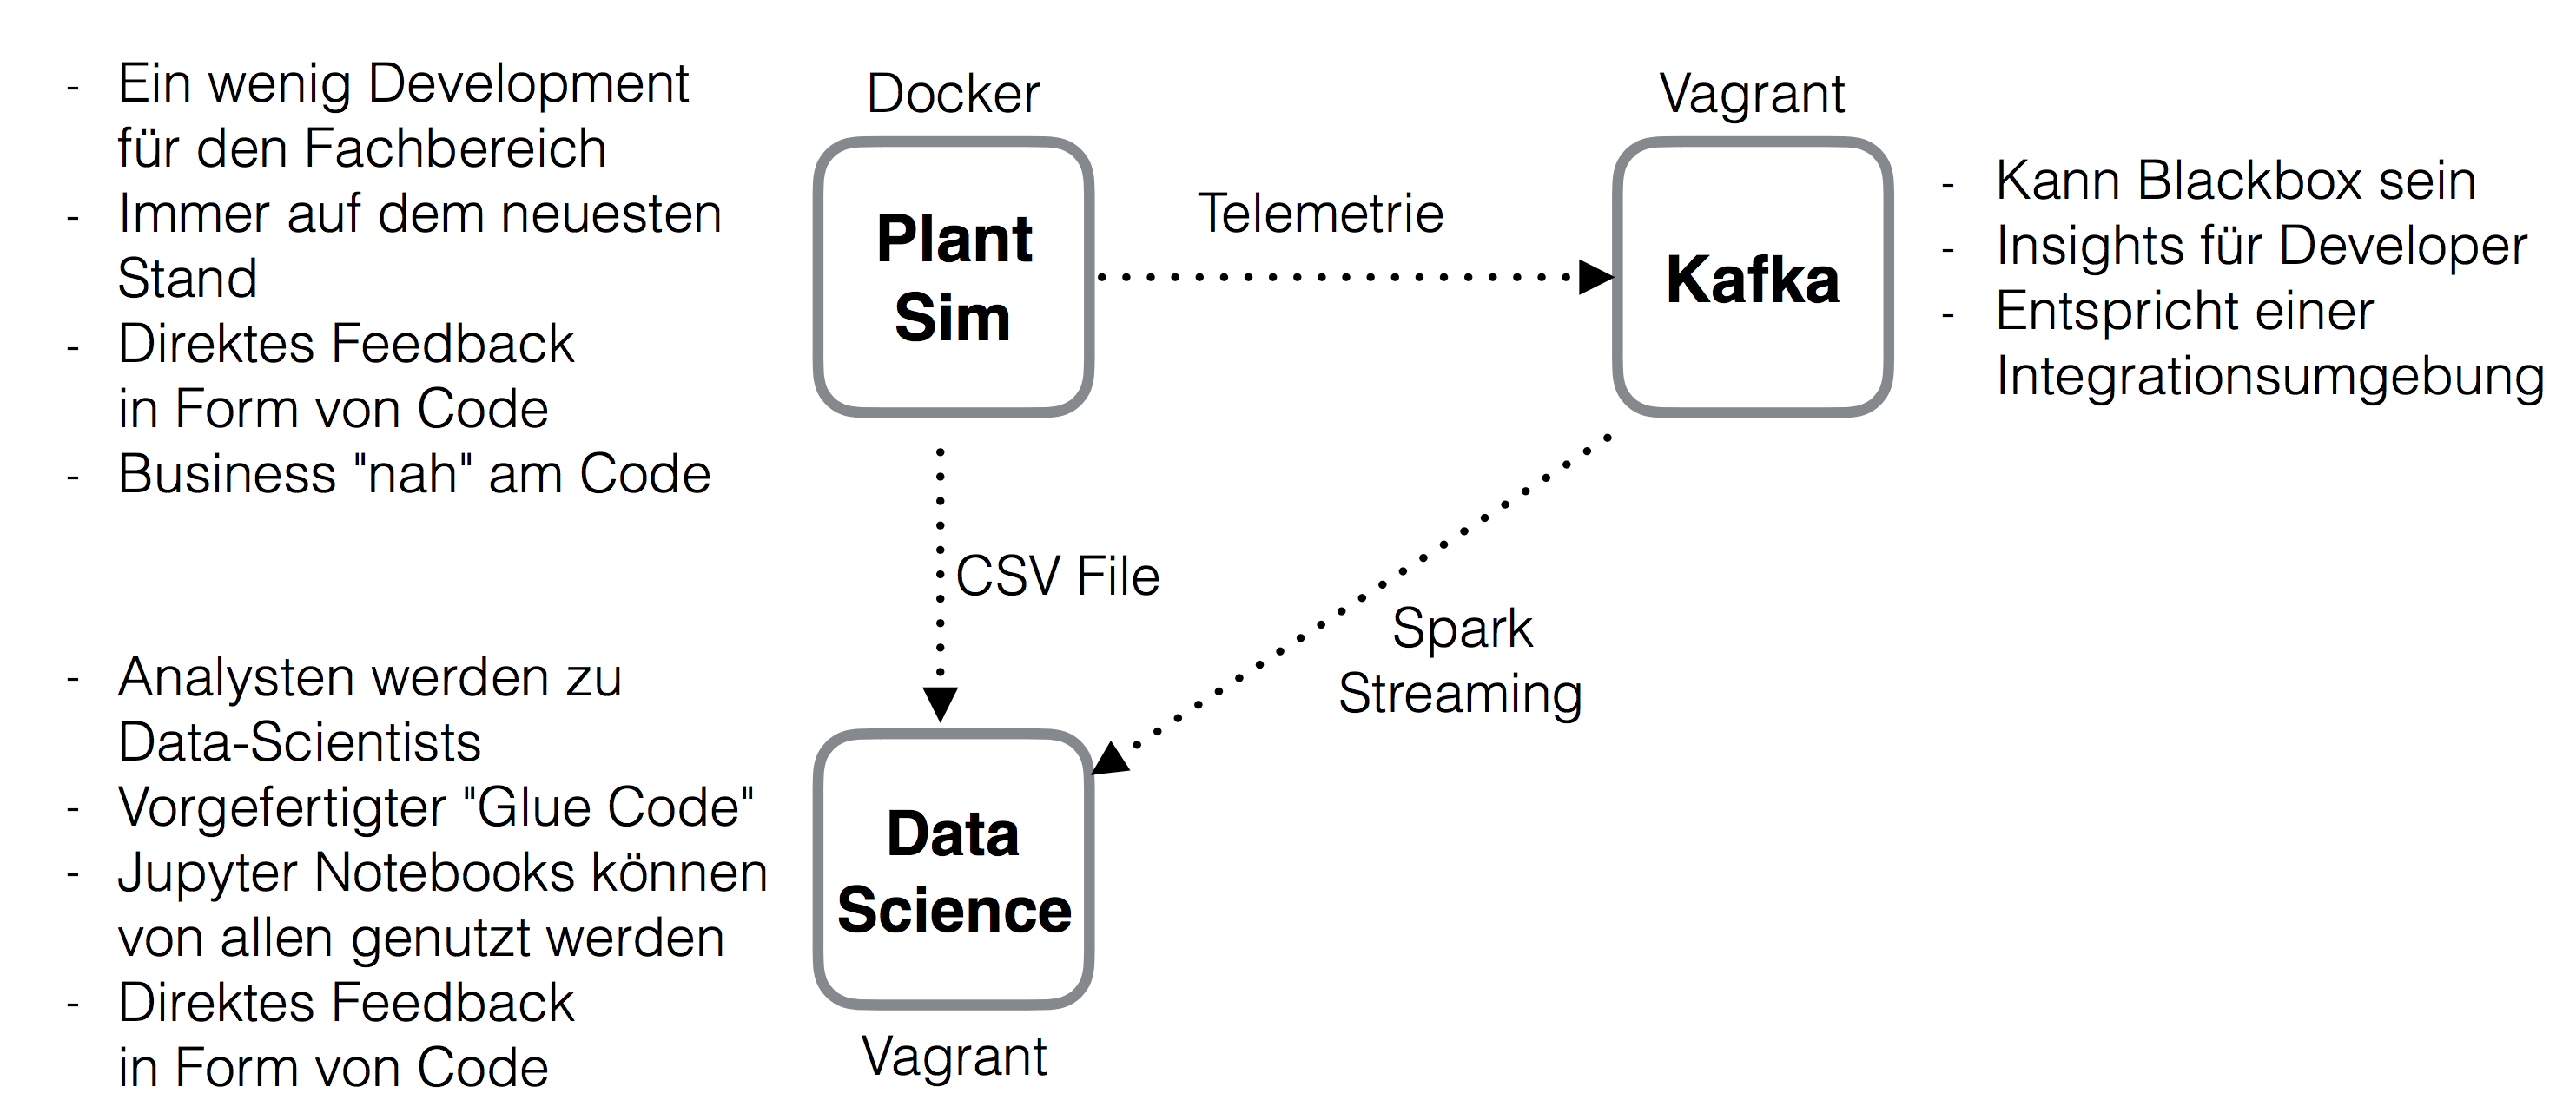
\includegraphics[width=1\textwidth,
  keepaspectratio=true]{bilder/data_science_all.png}
\end{frame}
